\documentclass[review,12pt]{elsarticle}
% Working draft. Methods (Sects. 2-5) follow the code in ../rovc; results (Sect. 6)
% are filled from ../results by hand and marked \todo where still open.

\usepackage{amsmath,amssymb}
\usepackage{booktabs}
\usepackage{graphicx}
\usepackage{xcolor}
\usepackage[hidelinks]{hyperref}
\usepackage{siunitx}
\graphicspath{{../figs/}}

\newcommand{\todo}[1]{\textcolor{red}{[TODO: #1]}}
\newcommand{\R}{\mathbb{R}}
\newcommand{\bnu}{\boldsymbol{\nu}}
\newcommand{\beeta}{\boldsymbol{\eta}}
\newcommand{\btau}{\boldsymbol{\tau}}
\newcommand{\pmNomMin}{45.0}
\newcommand{\pmNomMax}{52.3}
\newcommand{\dmNomMin}{43}
\newcommand{\dmNomMax}{60}
\newcommand{\pmSlowMin}{20.2}
\newcommand{\pmUncMin}{3.8}
\newcommand{\pmUncMax}{24.7}
\newcommand{\JuncZeroMin}{75}
\newcommand{\JuncZeroMax}{99}
\newcommand{\JuncThreeMin}{180}
\newcommand{\JuncThreeMax}{466}
\newcommand{\JuncSixMin}{422}
\newcommand{\JuncSixMax}{1314}
\newcommand{\JconZero}{133.5}
\newcommand{\JconSix}{138.1}


\journal{Ocean Engineering}

\begin{document}

\begin{frontmatter}

\title{Six-degree-of-freedom cascaded fractional-order control of an over-actuated ROV: margin-constrained tuning and a bias-controlled comparison of metaheuristics}

\author[1]{Hakan Ersoy\corref{cor}}
\cortext[cor]{Corresponding author.}
\author[1]{\todo{co-authors}}
\affiliation[1]{organization={\todo{affiliation}}}

\begin{abstract}
Fractional-order controllers for remotely operated vehicles are mostly designed for one axis, with idealized
thrusters and no latency. We recast the cascaded FOPID-(1+TFOID) controller, proposed for load-frequency
control, as a position--velocity cascade for all six degrees of freedom of an over-actuated BlueROV2 Heavy with
eight T200 thrusters, whose thrust, dead band, saturation and electrical power are fitted to the manufacturer's
measurements. Tuning minimizes a multi-scenario six-DOF ITAE and energy cost subject to phase margins on every
linearized loop over a range of thruster lag (0.05--0.2~s) and latency (10--60~ms). Six metaheuristics,
including the recent stellar oscillation optimizer (SOO), are compared at an equal evaluation budget and in a
mirrored search box: particle swarm optimization gives the lowest median cost, unchanged in the mirrored box,
while SOO and golden jackal optimization are attracted to the coordinate origin. Over 120 tuning runs on nominal
cases, a lower training cost goes with more divergences in a 100-draw Monte Carlo study of plant and actuator
parameters, for every cascade. With a robust training set that adds a severe-noise case and a weak-actuator
case, none of the 40 cascade tunings diverges, and the proposed cascade is the best structure: its median
training cost is 36\% below that of a tuned integer P-PID cascade ($p=0.026$), with 35\% less error in a
multi-set-point storm test and three times less under severe sensor noise. Tuning without latency and margin
constraints gives margins down to \pmUncMin$^\circ$ and a storm-test cost 1.8--5.6 times higher at 30~ms of
latency.
\end{abstract}

\begin{highlights}
\item Cascaded FOPID-(1+TFOID) control of all six DOF of an over-actuated BlueROV2 Heavy
\item Phase margins are imposed over a range of thruster lag and latency during tuning
\item Tuning on nominal cases trades robustness for nominal cost in every cascade
\item With robust tuning, the fractional cascade beats the P-PID cascade by 35\% in storms
\item Equal budgets and a mirrored search box expose the origin bias of SOO and GJO
\end{highlights}

\begin{keyword}
remotely operated vehicle \sep fractional-order control \sep cascade control \sep FOPID \sep tilt-integral-derivative
\sep metaheuristic tuning \sep phase margin \sep BlueROV2
\end{keyword}

\end{frontmatter}

%% ---------------------------------------------------------------------------
\section{Introduction}\label{sec:intro}

\todo{Paragraph 1: ROV/AUV motion control, coupled nonlinear hydrodynamics, wave and current disturbances;
most FO studies regulate a single axis.}

\todo{Paragraph 2: our earlier study \cite{ersoy2026jestech}: surge-axis PI$^\lambda$D$^\mu$ \cite{podlubny1999},
fourth-order plant identified from T200 measurements, PSO \cite{kennedy1995pso} and DE \cite{storn1997de}
over a multi-scenario cost, four tests, FPGA realization. Limits: one axis, no coupling, no allocation,
no latency or margin requirement.}

\todo{Paragraph 3: cascaded FO controllers in load-frequency control; FOPID-(1+TFOID) of
\cite{nour2026scirep} with SOO \cite{rodan2025soo}; its own stated limits (no formal stability analysis,
simulation only).}

\todo{Paragraph 4: tuning by new metaheuristics; equal-iteration comparisons that give some methods twice the
evaluations; origin/centre bias \cite{kudela2022,camacho2023}; inconsistencies between the SOO paper and its
code \cite{mealpy_soo}.}

The contributions of this paper are:
\begin{enumerate}
\item The FOPID-(1+TFOID) cascade is recast as a position--velocity cascade (the second stage acts on
  $u_1-\nu$, the mechanical counterpart of $u_1-\Delta f$) and applied to all six DOF of an over-actuated
  BlueROV2 Heavy, with six benchmark structures realized in the same cascade form.
\item Tuning is subject to phase margins on every linearized DOF loop, imposed over a range of thruster lag and
  latency because the T200 dynamics are not known well. Without them, ITAE tuning returns loops with margins
  below \SI{10}{\degree} that one or two extra samples of latency destabilize (Sect.~\ref{sec:latency}).
\item We show that tuning on nominal cases trades robustness for nominal cost: over 120 runs, a lower nominal
  training cost goes with more divergences in a Monte Carlo study, for every cascade. Adding a severe-noise case
  and a weak-actuator case to the training set removes the divergences of all structures; under this robust
  tuning the proposed cascade is the best structure, significantly better than the integer P-PID cascade.
\item The thruster model (thrust, dead band, asymmetry, saturation and electrical power at 10--20~V) is fitted
  to the manufacturer's measurements \cite{t200data}, so the effort term is energy in joules and battery
  voltage is a physically meaningful uncertainty.
\item Six tuners, including the newest (SOO), are compared at an equal evaluation budget, in the original
  and in a mirrored search box, and on shifted benchmark functions; this separates search ability from
  attraction to the coordinate origin.
\end{enumerate}

%% ---------------------------------------------------------------------------
\section{Vehicle and actuator model}\label{sec:model}

\subsection{Rigid-body and hydrodynamic model}
Let $\beeta=[x,y,z,\phi,\theta,\psi]^\top$ be the position and attitude in the north-east-down frame
and $\bnu=[u,v,w,p,q,r]^\top$ the velocities in the body frame, whose origin is the centre of gravity.
The vehicle obeys \cite{fossen2011}
\begin{equation}\label{eq:plant}
\begin{aligned}
  \boldsymbol{M}\dot{\bnu} + \boldsymbol{C}_{RB}(\bnu)\bnu + \boldsymbol{C}_{A}(\bnu_r)\bnu_r
  + \boldsymbol{D}(\bnu_r)\bnu_r + \boldsymbol{g}(\beeta) &= \boldsymbol{T}\boldsymbol{f} + \btau_d,\\
  \dot{\beeta} &= \boldsymbol{J}(\beeta)\bnu,
\end{aligned}
\end{equation}
where $\boldsymbol{M}=\boldsymbol{M}_{RB}+\boldsymbol{M}_A$ is diagonal, $\bnu_r=\bnu-[\boldsymbol{R}^\top
\boldsymbol{v}_c;\boldsymbol{0}]$ is the velocity relative to an irrotational current $\boldsymbol{v}_c$
(the term $\boldsymbol{M}_A\dot{\bnu}_c$ is neglected), $\boldsymbol{D}(\bnu_r)=\boldsymbol{D}_l+
\boldsymbol{D}_q\,\mathrm{diag}(|\bnu_r|)$, and $\boldsymbol{g}$ contains the restoring forces of the weight and
buoyancy. The parameters of the heavy configuration are those of the open benchmark of
\cite{vonbenzon2022} (Table~\ref{tab:params}).

\begin{table}[t]
\centering\small
\caption{BlueROV2 Heavy parameters \cite{vonbenzon2022}.}\label{tab:params}
\resizebox{\textwidth}{!}{%
\begin{tabular}{llll}
\toprule
mass $m$ & \SI{13.5}{kg} & volume $\nabla$ & \SI{0.0135}{m^3} (neutral) \\
$I_x, I_y, I_z$ & 0.26, 0.23, 0.37~\si{kg.m^2} & $\boldsymbol{r}_b$ & $[0,0,-0.01]$~m \\
added mass & \multicolumn{3}{l}{$X_{\dot u}$ 6.357, $Y_{\dot v}$ 7.121, $Z_{\dot w}$ 18.69~kg;
  $K_{\dot p}$ 0.1858, $M_{\dot q}$ 0.1348, $N_{\dot r}$ 0.2215~\si{kg.m^2}} \\
linear damping & \multicolumn{3}{l}{$X_u$ 13.7, $Y_v$ 0, $Z_w$ 33~\si{N.s/m}; $K_p$ 0, $M_q$ 0.8, $N_r$ 0~\si{N.m.s/rad}} \\
quadratic damping & \multicolumn{3}{l}{$X_{u|u|}$ 141, $Y_{v|v|}$ 217, $Z_{w|w|}$ 190~\si{N.s^2/m^2};
  $K_{p|p|}$ 1.192, $M_{q|q|}$ 0.47, $N_{r|r|}$ 1.5~\si{N.m.s^2/rad^2}} \\
\bottomrule
\end{tabular}}
\end{table}

\subsection{Thrusters and allocation}
Four horizontal thrusters at \SI{45}{\degree} and four vertical thrusters give the $6\times 8$ allocation
matrix $\boldsymbol{T}$ of \cite{vonbenzon2022}. A demanded generalized force $\btau$ is distributed by
$\boldsymbol{f}_d=\boldsymbol{T}^{+}\btau$ and scaled down as a whole when a thruster limit is reached, so
the direction of $\btau$ is kept. Each command is mapped to a normalized PWM value $u_i\in[-1,1]$ by the
inverse of the nominal \SI{16}{V} curve, with dead-band compensation. The thrust produced is
\begin{equation}
  F(u)=\begin{cases} \sum_{k=1}^{3} a_k (u-d_+)^k, & u>d_+,\\ 0, & -d_-\le u\le d_+,\\
  -\sum_{k=1}^{3} b_k (-u-d_-)^k, & u<-d_-,\end{cases}
\end{equation}
followed by a first-order lag $\tau_m$. No reliable dynamic model of the T200 is available: the
manufacturer estimates 25--40~ms of ESC latency for a running motor, and about 110~ms has been reported from
standstill. We therefore take $\tau_m=\SI{0.1}{s}$ and a latency of \SI{30}{ms} as nominal values and
design for $\tau_m\in[0.05,0.2]$~s and latencies of 10--60~ms (Sect.~\ref{sec:tuning}). The coefficients were fitted by least squares to the manufacturer's
measurements at 10--20~V \cite{t200data}; at \SI{16}{V} the fit error is \SI{0.24}{N} RMS (\SI{1.3}{N}
maximum) over the range \SIrange{-39.9}{51.4}{N}. The electrical power of the actual thrust,
$P(F)=\sum_k q_k|F|^k$, is fitted to the same data (\SI{3.1}{W} RMS of \SI{389}{W}). The command reaches the
thrusters three control periods ($3\Delta t=\SI{30}{ms}$) after the measurement it was computed from.

\subsection{Disturbances and navigation errors}
Waves act as a sum of five sinusoids per DOF with random frequencies in \SIrange{0.4}{1.6}{rad/s}
(amplitudes 20, 20, 15~N and 1~N\,m), and a current of \SI{0.25}{m/s} ($\pm 20\%$ slow variation)
acts through $\bnu_r$. The controller sees the output of a navigation filter, modelled as first-order
Gauss--Markov errors with \SI{2}{Hz} bandwidth (one sigma: position \SI{1}{cm}, depth \SI{5}{mm},
attitude 0.17--\SI{0.29}{\degree}, velocity \SI{1}{cm/s}, rates \SI{0.29}{\degree/s}).

%% ---------------------------------------------------------------------------
\section{Controller}\label{sec:controller}

\subsection{Position--velocity form of the FOPID-(1+TFOID)}
For each DOF $i$, the first stage acts on the position error $e_{1,i}$ (expressed in the body frame for
the translational DOFs) and returns a velocity reference,
\begin{equation}\label{eq:stage1}
  u_{1,i}(s) = \Big(K_p + \frac{K_{i1}}{s^{\lambda_1}} + K_{d1}s^{\mu_1}\Big) e_{1,i}(s).
\end{equation}
The second stage acts on $e_{2,i}=u_{1,i}-\nu_i$ and returns an acceleration demand,
\begin{equation}\label{eq:stage2}
  a_i(s) = \Big(1 + \frac{K_t}{s^{1/n}} + \frac{K_{i2}}{s^{\lambda_2}} + K_{d2}s^{\mu_2}\Big) e_{2,i}(s),
  \qquad \tau_i = M_{ii}\, a_i .
\end{equation}
In \cite{nour2026scirep} the second stage acts on $u_1-\Delta f$; here the local feedback is the measured
velocity, which makes the cascade a position--velocity cascade in the usual sense of marine control.
Scaling by the nominal inertia $M_{ii}$ makes the gains dimensionally consistent across DOFs. One parameter
set is shared by $(x,y,z)$ and one by $(\phi,\theta,\psi)$: 22 decision variables.

\subsection{Benchmark structures}
Table~\ref{tab:structures} lists the six benchmarks. FOPID is the single-loop PI$^\lambda$D$^\mu$ of
\cite{ersoy2026jestech} extended to six DOF, P-PID the integer cascade of common ROV autopilots, and the
three fractional cascades are those compared in \cite{nour2026scirep}. All cascades use the
position--velocity form of Eqs.~\eqref{eq:stage1}--\eqref{eq:stage2}, so the comparison isolates the stage
transfer functions.

\begin{table}[t]
\centering\small
\caption{Controller structures. $G_1$ acts on the position error; $G_2$ on $u_1-\nu$ (cascades only).
Decision variables: two groups (translation, rotation).}\label{tab:structures}
\resizebox{\textwidth}{!}{%
\begin{tabular}{lllr}
\toprule
structure & $G_1(s)$ & $G_2(s)$ & variables \\
\midrule
FOPID-(1+TFOID) (proposed) & $K_p + K_{i1}s^{-\lambda_1} + K_{d1}s^{\mu_1}$ & $1 + K_t s^{-1/n} + K_{i2}s^{-\lambda_2} + K_{d2}s^{\mu_2}$ & 22 \\
FOPID \cite{ersoy2026jestech} & $K_p + K_i s^{-\lambda} + K_d s^{\mu}$ & -- & 10 \\
PID & $K_p + K_i/s + K_d s/(s/\omega_h+1)$ & -- & 6 \\
P-PID & $K_{p1}$ & $K_{p2} + K_{i2}/s + K_{d2}s/(s/\omega_h+1)$ & 8 \\
PI-(1+FOPID) & $K_{p1} + K_{i1}/s$ & $1 + K_{p2} + K_{i2}s^{-\lambda} + K_d s^{\mu}$ & 14 \\
FOPID-FOPI & $K_{p1} + K_{i1}s^{-\lambda_1} + K_d s^{\mu}$ & $K_{p2} + K_{i2}s^{-\lambda_2}$ & 16 \\
FOPI-FOPD & $K_{p1} + K_i s^{-\lambda}$ & $K_{p2} + K_d s^{\mu}$ & 12 \\
\bottomrule
\end{tabular}}
\end{table}

\subsection{Realization}
Each $s^{\alpha}$ is approximated by the Oustaloup filter \cite{oustaloup2000} of order $N=5$ on
\SIrange{e-3}{e2}{rad/s}; for $\alpha<-1$ an exact integrator is split off. Every first-order section is
discretized by the Tustin rule at $\Delta t=\SI{10}{ms}$. Integer derivatives use the same high-frequency
limit, $K_d s/(s/\omega_h+1)$ with $\omega_h=\SI{100}{rad/s}$. The reference passes a critically damped
second-order model with $\omega=\SI{1}{rad/s}$, identical for all structures.

%% ---------------------------------------------------------------------------
\section{Tuning problem}\label{sec:tuning}

\subsection{Cost}
The \emph{nominal} training set has two cases, whose disturbance and noise realizations differ from those of
the tests: a simultaneous step in $x$, $y$, $z$ and $\psi$ (\SI{20}{s}), and station keeping in waves and
current with steps in $\psi$ and $z$ (\SI{30}{s}). The \emph{robust} training set adds a step under severe
white sensor and process noise (the noise model of test T2, another realization, \SI{15}{s}) and a corner case
in waves with a weak actuator and a heavier vehicle (\SI{12}{V} battery, $\tau_m=\SI{0.2}{s}$, \SI{60}{ms},
added mass $\times1.5$, \SI{20}{s}). The cost is
\begin{equation}\label{eq:cost}
  J = \sum_{s}\Big[\sum_{i=1}^{6} w_i\int_0^{T_s} t\,|e_i(t)|\,dt + \rho E_s\Big]
      + K_{pm}\sum_{a}\sum_{i=1}^{6}\frac{\max(0,\ \mathrm{PM}_a^\ast-\mathrm{PM}_{a,i})}{\mathrm{PM}_a^\ast},
\end{equation}
with $w=[1,1,1,2,2,2]$ (one metre of error weighs as much as \SI{0.5}{rad}), the electrical energy $E_s$ in
joules, $\rho=\num{2e-4}\,\si{J^{-1}}$ and $K_{pm}=200$. The margins are required at three actuator points $a$:
the nominal thruster ($\tau_m=\SI{0.1}{s}$, \SI{30}{ms}; $\mathrm{PM}^\ast=\SI{45}{\degree}$) and the slow
(\SI{0.2}{s}, \SI{60}{ms}) and fast (\SI{0.05}{s}, \SI{10}{ms}) corners ($\mathrm{PM}^\ast=\SI{20}{\degree}$).
Diverging runs receive $10^4(1+\text{lost fraction})$.

\subsection{Margin constraint}
About hover, DOF $i$ is $\ddot y + c_{1,i}\dot y + c_{0,i}y = H(s)a$ with $c_1=D_{l,ii}/M_{ii}$ and the
restoring stiffness $c_0=z_bB/M_{ii}$ in roll and pitch. The actuator path
$H(s)=e^{-(n_d+1/2)\Delta t s}/(\tau_m s+1)$ contains $n_d$ periods of latency, the zero-order hold and the
thruster lag. Broken at $a$, the loop is
\begin{equation}
  L_i(s) = G_2(s)\big(G_1(s)+s\big)P_i(s), \qquad P_i(s) = \frac{H(s)}{s^2+c_{1,i}s+c_{0,i}},
\end{equation}
($L_i=G_1P_i$ for single-loop structures), with $G_1,G_2$ the stage transfer functions as realized
(Oustaloup). $\mathrm{PM}_i$ is the smallest distance of $\arg L_i$ from \SI{-180}{\degree} over all gain
crossovers below \SI{300}{rad/s}; a loop whose crossover lies above (the Nyquist frequency is
\SI{314}{rad/s}) gets $\mathrm{PM}_i=\SI{-180}{\degree}$. The linear analysis predicts the latency at which
the simulated loop loses stability (unit test \texttt{test\_margins\_predict\_simulated\_delay\_limit}).

\subsection{Search space}
Gains are searched as $\log_{10}K\in[-2,\log_{10}50]$, the orders as $\lambda\in[0,1.5]$, $\mu\in[0,1]$, and
$n\in[1,10]$. On a linear gain scale most random initial points violate the margin constraint and all
tuners stalled near $J\approx100$.

%% ---------------------------------------------------------------------------
\section{Tuners and comparison protocol}\label{sec:tuners}

\subsection{Stellar oscillation optimizer}
SOO \cite{rodan2025soo} moves a population of $N$ oscillators in two stages per iteration $t=1,\dots,T$.
With the angular frequency $\omega(t)=2\pi/(P_0+\Delta P\,t)$, the scaling factor $S(t)=2(1-t/T)$, the best
position $\boldsymbol{x}_b$ and $r_1,r_2,r_3\sim U(0,1)$ drawn per component, the first stage forms
\begin{align}
  \boldsymbol{x}_{o1} &= \boldsymbol{x}_b - r_1 r_3 S(\omega r_1-1)\big(\boldsymbol{x}_i - |r_1\sin(r_2)\,|r_3\boldsymbol{x}_b||\big),\label{eq:soo1}\\
  \boldsymbol{x}_{o2} &= \boldsymbol{x}_b - r_2 r_3 S(\omega r_1-1)\big(\boldsymbol{x}_i - |r_1\cos(r_2)\,|r_3\boldsymbol{x}_b||\big),\\
  \boldsymbol{x}_{new} &= r_3\,(\boldsymbol{x}_{o1}+\boldsymbol{x}_{o2})/2,\label{eq:soo3}
\end{align}
and the second stage moves each oscillator about the mean $\bar{\boldsymbol{x}}_3$ of the three best,
\begin{equation}
  \boldsymbol{x}_{osc} = \bar{\boldsymbol{x}}_3 + \tfrac12\big[\sin(r\pi)(\boldsymbol{x}_{a}-\boldsymbol{x}_{b'})
  + \cos((1-r)\pi)(\boldsymbol{x}_{a}-\boldsymbol{x}_{c})\big],
\end{equation}
with three other oscillators $a,b',c$, keeping each component of the old position with probability 1/2. We
follow the equations of the paper as read by the reimplementation in \cite{mealpy_soo}: both stages in every
iteration with greedy survivor selection, $P_0=3$, $\Delta P=0.001$, clipping at the bounds. That source
documents several differences between the paper and the authors' released code. SOO therefore spends $2N$
evaluations per iteration.

Eqs.~\eqref{eq:soo1}--\eqref{eq:soo3} refer to the coordinate origin twice: through $|r_3\boldsymbol{x}_b|$ and
through the factor $r_3\in[0,1]$, which contracts every candidate towards $\boldsymbol{0}$. As a control we use
\emph{BC-SOO}, the same first stage written in coordinates relative to $\boldsymbol{x}_b$ (the substitution
$\boldsymbol{x}\mapsto\boldsymbol{x}-\boldsymbol{x}_b$),
\begin{equation}
\begin{aligned}
  \boldsymbol{x}_{ok} &= \boldsymbol{x}_b - r_k r_3 S(\omega r_1-1)(\boldsymbol{x}_i-\boldsymbol{x}_b),\quad k=1,2,\\
  \boldsymbol{x}_{new} &= \boldsymbol{x}_b + r_3\big((\boldsymbol{x}_{o1}+\boldsymbol{x}_{o2})/2-\boldsymbol{x}_b\big),
\end{aligned}
\end{equation}
which is translation invariant by construction.

\subsection{Other tuners}
PSO with the constriction coefficients of \cite{clerc2002} ($w=0.7298$, $c_1=c_2=1.49618$, velocity limited to
20\% of the range), DE/rand/1/bin \cite{storn1997de} ($F=0.5$, $CR=0.9$), GWO \cite{mirjalili2014gwo}, GJO
\cite{chopra2022gjo} and uniform random search (RS). PSO and DE are the tuners of \cite{ersoy2026jestech};
GWO and GJO are among the comparison methods of \cite{nour2026scirep}.

\subsection{Protocol}
\begin{itemize}
\item \emph{Equal budget.} Every run stops after 3030 evaluations (population 30): 100 iterations for the
  one-stage methods and 50 for SOO. The equal-iteration protocol of \cite{nour2026scirep}, which gives SOO
  6030 evaluations, is run as a separate setting (SOO-iter).
\item \emph{Mirrored box.} Every tuner is also run on the problem expressed in the coordinates
  $\boldsymbol{x}'=\boldsymbol{lb}+\boldsymbol{ub}-\boldsymbol{x}$. The problem is the same; only the position of
  the coordinate origin relative to the good region changes. A tuner without positional bias gives the same
  distribution of results in both boxes.
\item \emph{Shifted benchmarks.} Sphere, Rastrigin, Rosenbrock and Ackley functions in $D=22$ on
  $[-100,100]^{22}$, with the optimum at the origin and at a random point of $[-60,60]^{22}$ (15 runs).
\item Ten independent runs per setting; medians, interquartile ranges and two-sided Mann--Whitney tests.
\end{itemize}

%% ---------------------------------------------------------------------------
\section{Results}\label{sec:results}

\subsection{Positional bias on shifted benchmarks}
\begin{figure}[t]
\centering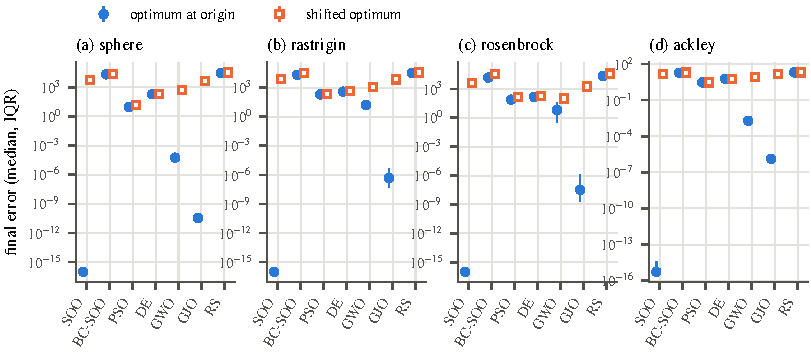
\includegraphics[width=\textwidth]{fig_x0_bias.pdf}
\caption{Final error after 3030 evaluations ($D=22$, box $[-100,100]^{22}$, 15 runs; median and
interquartile range) with the optimum at the origin (filled) and at a random point in $[-60,60]^{22}$
(open). Values below $10^{-15}$ are drawn at $10^{-16}$.}\label{fig:x0}
\end{figure}
With the optimum at the origin, SOO reaches $10^{-49}$ on the sphere and exactly zero on Rastrigin and
Rosenbrock; with the optimum shifted it ends at $6\times10^{3}$, $8\times10^{3}$ and $4\times10^{3}$
(Fig.~\ref{fig:x0}). GJO and GWO show the same pattern with smaller gaps, while PSO and DE give the same errors
in both cases, as expected from their translation-invariant updates. BC-SOO is translation invariant but
performs like random search: the search ability of SOO comes from its attraction to the origin.

\subsection{Tuners on the six-DOF problem}
\begin{table}[t]
\centering\small
\caption{Training cost $J$ of the proposed controller for ten runs per tuner (3030 evaluations unless
noted). $p$: two-sided Mann--Whitney tests against PSO (original box) and between the two boxes.}\label{tab:x1}
\resizebox{\textwidth}{!}{\begin{tabular}{lrllrr}
\toprule
tuner & best & median [IQR], original box & median [IQR], mirrored box & $p$ vs PSO & $p$ boxes \\
\midrule
PSO & 35.8 & 40.0 [37.9, 56.2] & 40.4 [38.9, 46.1] & -- & 1.000 \\
DE & 54.7 & 67.0 [58.3, 73.3] & 84.4 [56.4, 99.8] & 0.003 & 0.273 \\
GWO & 48.5 & 68.4 [55.9, 113.9] & 103.8 [84.9, 119.1] & 0.007 & 0.186 \\
SOO & 41.5 & 85.0 [69.6, 126.4] & 59.7 [52.6, 105.3] & 0.002 & 0.385 \\
SOO, 6030 eval. & 32.1 & 60.7 [43.4, 80.3] & -- & 0.089 & -- \\
GJO & 57.5 & 122.3 [90.7, 142.0] & 208.0 [165.8, 228.6] & $<0.001$ & 0.002 \\
BC-SOO & 215.8 & 329.8 [275.1, 410.9] & 325.3 [186.1, 435.1] & $<0.001$ & 0.521 \\
RS & 193.7 & 403.8 [279.5, 496.1] & 363.1 [321.8, 412.6] & $<0.001$ & 0.623 \\
\bottomrule
\end{tabular}
}
\end{table}
\begin{figure}[t]
\centering
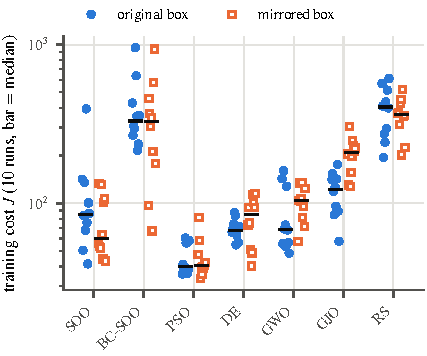
\includegraphics[width=0.49\textwidth]{fig_x1_runs.pdf}\hfill
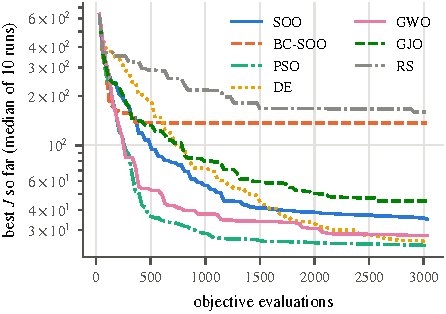
\includegraphics[width=0.49\textwidth]{fig_x1_convergence.pdf}
\caption{Left: training cost of every run in the original and mirrored boxes (bar: median). Right: median
best-so-far cost against the number of evaluations (original box).}\label{fig:x1}
\end{figure}
PSO gives the lowest median cost and the same distribution in both boxes (Table~\ref{tab:x1},
Fig.~\ref{fig:x1}). SOO is significantly worse than PSO at the same budget; with the equal-iteration protocol,
which doubles its evaluations, the difference is no longer significant ($p=0.089$) but its median stays 50\%
higher. GJO depends significantly on the box ($p=0.002$): its results change when only the position of the
coordinate origin relative to the good region changes. On this problem the origin of the search box is not
near the optimum (the gains are searched as $\log_{10}K$), so the attraction that makes SOO excel on centred
benchmarks no longer helps. PSO is used for the comparison of structures below; DE is kept as the second tuner
because it was the best tuner in \cite{ersoy2026jestech}.

\subsection{Nominal tuning trades robustness for nominal cost}
\begin{table}[t]
\centering\small
\caption{Training cost $J$ (PSO, ten runs per setting) and number of runs whose controller does not diverge in
any of the 100 Monte Carlo draws of T4 (no div.). Nominal: two training cases; robust: four. $J$ is comparable
within a column group only. $p$: Mann--Whitney test of the robust training cost against the proposed
cascade.}\label{tab:x2}
\resizebox{\textwidth}{!}{\begin{tabular}{lrrrrrrrr}
\toprule
 & \multicolumn{2}{c}{nominal, 3030} & \multicolumn{2}{c}{nominal, 10\,030} & \multicolumn{4}{c}{robust, 10\,030} \\ \cmidrule(lr){2-3}\cmidrule(lr){4-5}\cmidrule(lr){6-9}
structure & median $J$ & no div. & median $J$ & no div. & best $J$ & median $J$ & no div. & $p$ \\
\midrule
FOPID-(1+TFOID) & 40.0 & 5/10 & 36.9 & 4/10 & 70.6 & 80.4 & 10/10 & -- \\
PI-(1+FOPID) & 52.9 & 4/10 & 38.4 & 1/10 & 70.0 & 88.0 & 10/10 & 0.473 \\
P-PID & 70.1 & 5/10 & 65.0 & 5/10 & 89.0 & 125.3 & 10/10 & 0.026 \\
FOPI-FOPD & 56.2 & 8/10 & 50.6 & 6/10 & 79.9 & 127.3 & 10/10 & 0.045 \\
FOPID-FOPI & 315.6 & -- & 307.2 & -- & 650.9 & 665.6 & -- & $<0.001$ \\
FOPID & 388.9 & -- & 375.0 & -- & 853.2 & 914.1 & -- & $<0.001$ \\
PID & 639.6 & -- & 639.6 & -- & 975.0 & 975.0 & -- & $<0.001$ \\
\bottomrule
\end{tabular}
}
\end{table}
\begin{figure}[t]
\centering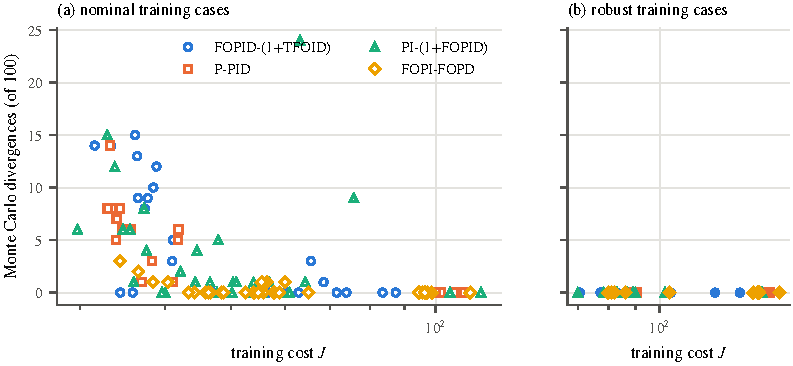
\includegraphics[width=\textwidth]{fig_tradeoff.pdf}
\caption{Training cost against the number of Monte Carlo divergences (of 100) for every run of the four
cascades. (a) Nominal training set, 3030 and 10\,030 evaluations (DE and PSO); (b) robust training set,
10\,030 evaluations (PSO). The costs of (a) and (b) are not comparable.}\label{fig:tradeoff}
\end{figure}
With the nominal training set and 3030 evaluations, the integer P-PID cascade reaches the lowest best training
cost (33.4 against 35.8 for the proposed cascade). With 10\,030 evaluations the fractional cascades pass it
(best 29.7 for PI-(1+FOPID), 31.5 for the proposed; median 36.9 for the proposed against 65.0 for P-PID), so
the gap at the smaller budget was a search limitation of the 22-parameter structure. The better-trained
controllers, however, are more fragile (Fig.~\ref{fig:tradeoff}a): over the 30 runs of each cascade, the rank
correlation between training cost and Monte Carlo divergences is $-0.92$ for P-PID, $-0.63$ for the proposed
cascade, $-0.45$ for PI-(1+FOPID) and $-0.44$ for FOPI-FOPD, and only 1--8 of 10 runs per setting are free of
divergence (Table~\ref{tab:x2}). The best nominal tuning of the proposed cascade diverges in 14 of 100 draws.
The optimizer exploits the nominal cases; robustness has to be part of the cost.

\subsection{Robust tuning: controller structures}
\begin{table}[t]
\centering\small
\caption{Test cases for the best robust tuning of each structure. Weighted ITAE as in Eq.~\eqref{eq:cost};
$E$: electrical energy in T4 (60~s); Monte Carlo: T4 with random mass ($\pm20\%$), added mass and damping
($\pm50\%$), buoyancy ($-2$ to $+3\%$), battery 12--20~V, thruster lag 0.05--0.2~s and latency
10--60~ms.}\label{tab:x3}
\resizebox{\textwidth}{!}{\begin{tabular}{lrrrrrrrr}
\toprule
 & \multicolumn{4}{c}{weighted ITAE} & $E$ T4 & \multicolumn{3}{c}{Monte Carlo, T4 (100)} \\ \cmidrule(lr){2-5}\cmidrule(lr){7-9}
structure (tuner) & T1 & T2 & T3 & T4 & [kJ] & median & p90 & diverged \\
\midrule
FOPID-(1+TFOID) (PSO) & 3.2 & 17.0 & 52.5 & 132.8 & 10.6 & 148 & 207 & 0 \\
PI-(1+FOPID) (PSO) & 4.4 & 22.0 & 50.2 & 160.1 & 10.6 & 172 & 213 & 0 \\
FOPI-FOPD (PSO) & 2.4 & 15.2 & 66.4 & 163.9 & 10.8 & 183 & 245 & 0 \\
P-PID (PSO) & 4.2 & 51.7 & 63.4 & 203.0 & 10.8 & 217 & 252 & 0 \\
FOPID-FOPI (PSO) & 25.1 & 37.9 & 384.6 & 1031.6 & 9.0 & 1093 & 1652 & 0 \\
FOPID (PSO) & 18.7 & 224.5 & 411.8 & 1039.6 & 10.0 & 1108 & 1662 & 0 \\
PID (PSO) & 16.8 & 127.4 & 1119.9 & 2553.8 & 10.0 & 2726 & 3710 & 0 \\
\bottomrule
\end{tabular}
}
\end{table}
\begin{figure}[t]
\centering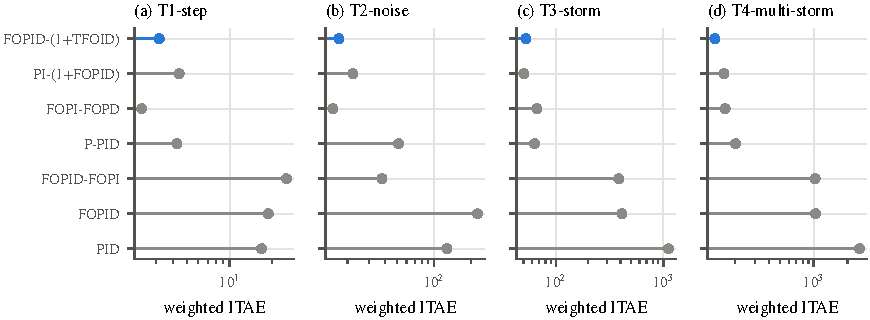
\includegraphics[width=\textwidth]{fig_x3_tests.pdf}
\caption{Weighted ITAE in the four test cases, best robust tuning of each structure (logarithmic
axes).}\label{fig:x3}
\end{figure}
\begin{figure}[t]
\centering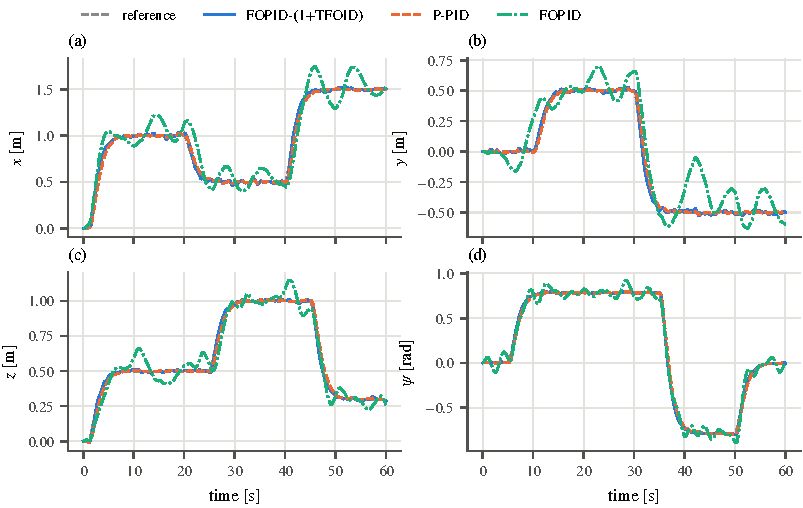
\includegraphics[width=\textwidth]{fig_t4_traces.pdf}
\caption{Test T4 (multi-level set points in waves and current): $x$, $y$, $z$ and $\psi$ for the proposed
cascade, the integer P-PID cascade and the single-loop FOPID of \cite{ersoy2026jestech}, each with its best
robust tuning.}\label{fig:t4}
\end{figure}
With the robust training set, none of the 40 cascade tunings diverges in the Monte Carlo study
(Fig.~\ref{fig:tradeoff}b). The proposed cascade has the lowest median training cost (80.4), significantly
below P-PID (125.3, $p=0.026$) and FOPI-FOPD (127.3, $p=0.045$) and on a par with PI-(1+FOPID) (88.0, $p=0.47$).
In the test cases (Table~\ref{tab:x3}, Fig.~\ref{fig:x3}) its best tuning has the lowest error in the
multi-set-point storm test T4 (132.8, 35\% below P-PID and 17\% below PI-(1+FOPID)), the lowest median and
90th percentile in the Monte Carlo study, and three times less error than P-PID under severe noise (T2).
Over all ten runs the differences to P-PID hold: median T4 cost 171.5 against 345.2 ($p=0.021$) and median T2
cost 14.2 against 33.7 ($p=0.003$). PI-(1+FOPID) is slightly better in the storm test T3 (50.2 against 52.5)
and FOPI-FOPD in T1 and T2, but both are worse in T4 and in the Monte Carlo study. The energy in T4 is the same
for all cascades within 2\%. The single-loop FOPID of \cite{ersoy2026jestech}, PID and FOPID-FOPI do not
diverge either, but they cannot reach a useful bandwidth within the margin constraints: their median training
costs are 8--12 times higher (Table~\ref{tab:x2}), their T4 errors 7.8--19 times higher than that of the
proposed cascade, and the vehicle oscillates in waves (Fig.~\ref{fig:t4}).

\subsection{Robustness}
\begin{figure}[t]
\centering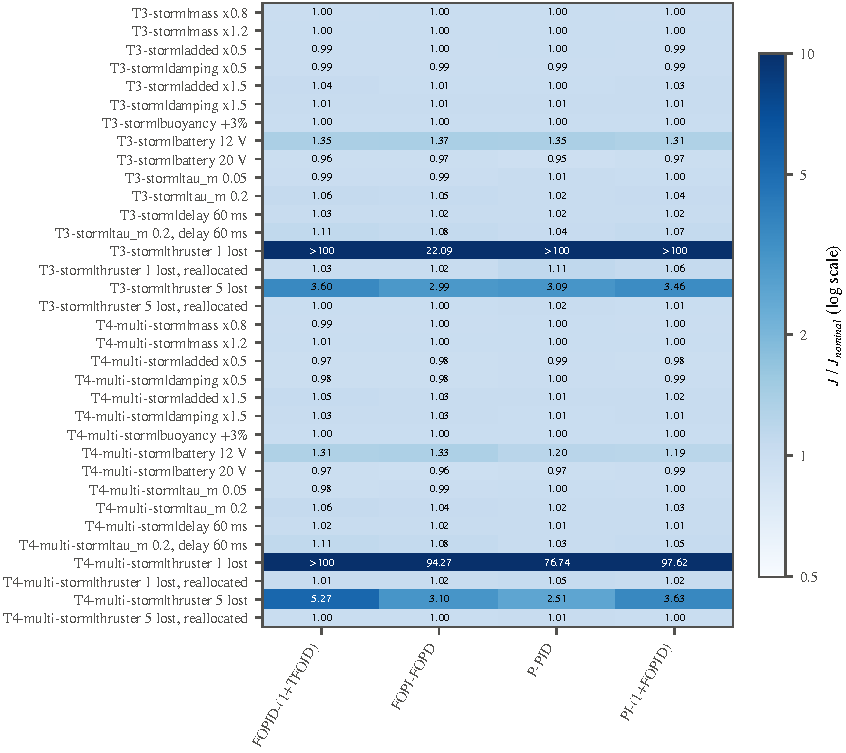
\includegraphics[width=0.8\textwidth]{fig_robustness.pdf}
\caption{Cost of each variant relative to the nominal test case, per structure, best robust tuning (the
controllers are not retuned).}\label{fig:rob}
\end{figure}
With robust tuning, mass, added mass, damping and buoyancy changes move the cost of the cascades by at most
5\% (Fig.~\ref{fig:rob}); a slow thruster with doubled latency costs 3--11\%. A \SI{12}{V} battery, which
lowers the maximum thrust by 28--29\% on the T200 curves, costs 19--37\%. Losing a horizontal thruster without
telling the allocation still makes the cascades diverge or degrade by more than 20 times, and losing a vertical
one costs 2.5--5.3 times. When
the failure is known and the allocation is recomputed on the remaining seven thrusters, the cost of the
proposed cascade rises by only 1--3\% (P-PID 5--11\%): the over-actuation of the heavy configuration is
useful only together with fault-aware allocation.

\subsection{Margins and latency}\label{sec:latency}
At the nominal thruster the six loops of the proposed controller (best robust tuning) have phase margins of
\pmNomMin--\pmNomMax$^\circ$ and tolerate \dmNomMin--\dmNomMax~ms of additional latency; at the slow corner the
smallest margin is \pmSlowMin$^\circ$, on the constraint. To show what the margin constraint buys, the proposed
controller was tuned as in the load-frequency study: no latency in the model and no margin requirement (X5,
six runs). The training cost drops to 18.6--22.2, but the smallest margin per run is
\pmUncMin--\pmUncMax$^\circ$. In T4 these controllers reach \JuncZeroMin--\JuncZeroMax{} without latency,
\JuncThreeMin--\JuncThreeMax{} at the nominal 30~ms and \JuncSixMin--\JuncSixMax{} at 60~ms, while the robust,
margin-constrained controller goes from \JconZero{} to \JconSix{} over the same range.

\section{Discussion and limitations}
\begin{itemize}
\item \emph{Robustness is a property of the tuning, not only of the structure.} With nominal training cases,
  every cascade can be tuned to a low nominal cost and a fragile controller; the comparison of structures is
  meaningful only when the cost contains the robustness requirement. Studies that tune on one nominal scenario
  (including \cite{ersoy2026jestech} and \cite{nour2026scirep}) may overstate the advantage of whichever
  structure their tuner happened to over-fit least.
\item \emph{Tuner choice.} The tuners were compared on the nominal cost (X1); PSO was then used for all
  structures. \todo{Repeat X1 with the robust training set in the final run.}
\item \emph{Thruster dynamics.} No validated dynamic model of the T200 was available; the design covers a
  range of lag and latency instead. \todo{Replace the nominal values by those of the MATLAB
  re-identification and narrow the range accordingly.}
\item \emph{Model.} Simulation only; hydrodynamic coefficients from \cite{vonbenzon2022}; one parameter
  set per group of DOFs; margins from a linearization about hover; navigation errors modelled, not estimated.
  Pool tests or hardware-in-the-loop, as in the FPGA realization of \cite{ersoy2026jestech}, are the next step.
\end{itemize}

\section{Conclusions}
We recast the FOPID-(1+TFOID) cascade as a position--velocity controller for all six DOF of an over-actuated
BlueROV2 Heavy with data-fitted T200 thrusters and tuned it under phase-margin constraints over a range of
thruster lag and latency. Compared at an equal budget and in a mirrored search box, PSO was the best tuner,
while the recent SOO and GJO showed a strong attraction to the coordinate origin. Tuning on nominal cases
produced controllers whose nominal cost and Monte Carlo robustness were inversely related; with a robust
training set no tuning of any cascade diverged, and the proposed cascade became the best structure, with 35\%
less error than the integer P-PID cascade in the multi-set-point storm test and three times less under severe
sensor noise. A known thruster failure costs it 1--3\% when the allocation is recomputed.

\section*{Data and code availability}
Code, results and figure scripts: \todo{repository URL}. The T200 data are fetched from the manufacturer and
checked by SHA-256 \cite{t200data}.

\bibliographystyle{elsarticle-num}
\bibliography{refs}

\end{document}
